\chapter{Capitolo 5}
\section{La necessità di sicurezza del database}
I database delle organizzazioni tendono a concentrare le informazioni sensibili in un unico sistema logico. Gli esempi includono:
\begin{itemize}
    \item Dati finanziari aziendali
    
    \item Registrazioni telefoniche riservate
    
    \item Informazioni sui clienti e sui dipendenti, come il nome, il numero di previdenza sociale, le informazioni sul conto bancario e le informazioni sulla carta di credito
    
    \item Informazioni proprietarie sui prodotti
    
    \item Informazioni sanitarie e cartelle cliniche 
\end{itemize}

Per molte aziende e altre organizzazioni è importante poter fornire a clienti, partner e dipendenti l'accesso a queste informazioni. Tuttavia, tali informazioni possono essere oggetto di minacce interne ed esterne di uso improprio o di modifiche non autorizzate. Di conseguenza, la sicurezza specifica per i database è una componente sempre più importante di una strategia di sicurezza organizzativa complessiva. 

\singlespacing

Le seguenti sono le ragioni per le quali la sicurezza dei database non ha tenuto il passo con la crescente dipendenza dai database:

\begin{enumerate}

    \item Esiste un drammatico squilibrio tra la complessità dei moderni sistemi di gestione dei database (DBMS) e le tecniche di sicurezza utilizzate per proteggere questi sistemi critici. Un DBMS è un software molto complesso e di grandi dimensioni, che offre molte opzioni, tutte da comprendere bene e da proteggere per evitare violazioni dei dati. Sebbene le tecniche di sicurezza siano progredite, la crescente complessità dei DBMS con molte nuove funzionalità e servizi, ha portato a una serie di nuove vulnerabilità e al potenziale uso improprio.
    
    \item I database dispongono di un sofisticato protocollo di interazione chiamato Structured Query Language (SQL), che è di gran lunga SQL (Structured Query Language), che è molto più complesso, ad esempio, del protocollo HTTP (Hypertext Transfer Protocol) utilizzato per interagire con un servizio Web. Una sicurezza efficace dei database richiede una strategia basata sulla piena comprensione delle vulnerabilità di sicurezza dell'SQL.
    
    \item L'organizzazione tipica non dispone di personale a tempo pieno per la sicurezza dei database. Il risultato è uno squilibrio tra requisiti e capacità. La maggior parte delle organizzazioni dispone di uno staff di amministratori di database, il cui compito è quello di gestire il database per garantire disponibilità, prestazioni, correttezza e facilità d'uso. Questi amministratori possono avere una conoscenza limitata della sicurezza e poco tempo a disposizione per padroneggiare e applicare le tecniche di sicurezza. D'altra parte, i responsabili della sicurezza all'interno di un'organizzazione possono avere una conoscenza molto limitata della tecnologia dei database e dei DBMS.
    
    \item La maggior parte degli ambienti aziendali è costituita da un mix eterogeneo di piattaforme di database (Oracle, IBM DB2).
\end{enumerate}
\section{Sistemi di gestione dei database}
Un database è una raccolta strutturata di dati memorizzati per essere utilizzati da una o più applicazioni. Oltre ai dati, un database contiene le relazioni tra i dati e i gruppi di dati. Come esempio della distinzione tra file di dati e database, si consideri quanto segue: Un semplice file del personale potrebbe consistere in una serie di record, uno per ogni dipendente. Ogni record riporta il nome, l'indirizzo, la data di nascita, la posizione, lo stipendio e altri dettagli necessari all'ufficio del personale.

\singlespacing

Un database del personale comprende un file del personale, come appena descritto. Può anche includere un file delle presenze, che mostra per ogni settimana le ore lavorate da ciascun dipendente. Con un'organizzazione a database, questi due file sono Questi due file sono collegati tra loro, in modo che un programma per le paghe possa estrarre le informazioni sulle ore lavorate e sulla retribuzione di ciascun dipendente e lo stipendio di ciascun dipendente per generare le buste paga. Il database è accompagnato da un sistema di gestione di database (DBMS), che è una suite di programmi per la costruzione di un sistema di gestione di database.

\singlespacing

\begin{figure}[H]
	\centering
    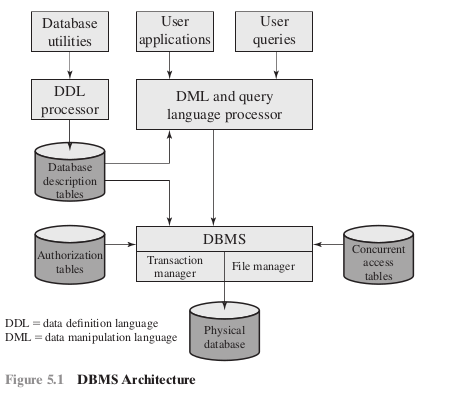
\includegraphics[width=14cm, keepaspectratio]{Bistarelli/img/cap_5/figura5.1.png}
\end{figure}

Un linguaggio di interrogazione fornisce un'interfaccia uniforme al database per utenti e applicazioni.
La Figura 5.1 mostra un diagramma a blocchi semplificato dell'architettura di un DBMS. I progettisti e gli amministratori di database utilizzano un linguaggio di definizione dei dati (DDL) per definire la struttura logica del database e le proprietà procedurali, che sono rappresentate da una serie di descrizioni del database. Un linguaggio di manipolazione dei dati (DML) fornisce un potente insieme di strumenti per gli sviluppatori di applicazioni. I linguaggi di interrogazione sono linguaggi dichiarativi progettati per supportare gli utenti finali. Il sistema di gestione del database utilizza le tabelle di descrizione del database per gestire il database fisico.
L'interfaccia al database avviene attraverso un modulo di gestione dei file e un modulo di gestione delle transazioni.
e un modulo di gestione delle transazioni. Oltre alla tabella di descrizione del database, altre due tabelle supportano il DBMS.

\singlespacing

Il DBMS utilizza tabelle di autorizzazione per garantire che l'utente abbia il permesso di eseguire la query. La tabella di accesso concorrente previene i conflitti quando vengono eseguiti comandi simultanei in conflitto. I sistemi di database forniscono un accesso efficiente a grandi volumi di dati e sono vitali per il funzionamento di molte organizzazioni. 

\section{Sql Injection Attacks}
L'attacco SQL injection (SQLi) è una delle minacce alla sicurezza della rete più diffuse e pericolose delle minacce alla sicurezza della rete. 

\singlespacing

Considerate i seguenti rapporti:

\begin{enumerate}
    \item Il rapporto sugli attacchi alle applicazioni Web di Imperva del luglio 2013 ha esaminato una sezione di server di applicazioni Web nel settore e ha monitorato otto diversi tipi di attacchi comuni. Il rapporto ha rilevato che gli attacchi SQLi si sono classificati al primo o al secondo posto per numero totale di attacchi, numero di richieste di attacco per ogni attacco e numero medio di giorni al mese in cui un'applicazione ha subito almeno un attacco. Imperva ha osservato un singolo sito web che ha ricevuto 94.057 richieste di attacco SQL injection in un solo giorno.
    
    \item Il rapporto 2013 dell'Open Web Application Security Project [OWAS13] sui 10 rischi più critici per la sicurezza delle applicazioni Web elenca gli attacchi a iniezione, in particolare gli attacchi SQLi, come il rischio principale.
    
    \item  Il rapporto Veracode 2016 State of Software Security ha rilevato che la percentuale di applicazioni colpite da attacchi SQLi si aggira intorno al 35\%.
    
    \item Il Trustwave 2016 Global Security Report [TRUS16] elenca gli attacchi SQLi come una delle due principali tecniche di intrusione. Il rapporto rileva che SQLi può rappresentare una minaccia significativa per i dati sensibili, come le informazioni di identificazione personale (PII) e i dati delle carte di credito, e può essere difficile prevenire e relativamente facile sfruttare questi attacchi.
\end{enumerate}

In termini generali, un attacco SQLi è progettato per sfruttare la natura delle pagine delle applicazioni Web.
pagine web. A differenza delle pagine web statiche degli anni passati, la maggior parte dei siti web attuali hanno componenti e contenuti dinamici. Molte di queste pagine richiedono informazioni, come informazioni, come la posizione, le informazioni sull'identità personale e i dati della carta di credito. 

\singlespacing

Questo contenuto dinamico viene solitamente trasferito da e verso database back-end che contengono volumi di informazioni, dai dati dei titolari di carta di credito al tipo di scarpe da corsa più acquistato. La pagina web di un server applicativo esegue query SQL ai database per inviare e ricevere informazioni fondamentali per rendere positiva l'esperienza dell'utente. In un ambiente di questo tipo, un attacco SQLi è progettato per inviare comandi SQL dannosi al server di database. L'obiettivo più comune dell'attacco è l'estrazione in blocco dei dati. Gli aggressori possono scaricare tabelle di database con centinaia di migliaia di record di clienti. A seconda dell'ambiente, l'iniezione SQL può essere sfruttata anche per modificare o eliminare dati, eseguire comandi arbitrari del sistema operativo o lanciare attacchi denial-of-service (DoS). 

\subsection{Un tipico attacco SQLi}
SQLi è un attacco che sfrutta una vulnerabilità di sicurezza che si verifica nel livello di database di un'applicazione (come le query). Utilizzando l'iniezione SQL, l'aggressore può estrarre o manipolare i dati dell'applicazione web.
L'attacco è attuabile quando l'input dell'utente viene filtrato in modo errato per i caratteri di escape letterali di stringa incorporati nelle istruzioni SQL oppure l'input dell'utente non è fortemente tipizzato e quindi viene eseguito inaspettatamente.

\begin{figure}[H]
	\centering
    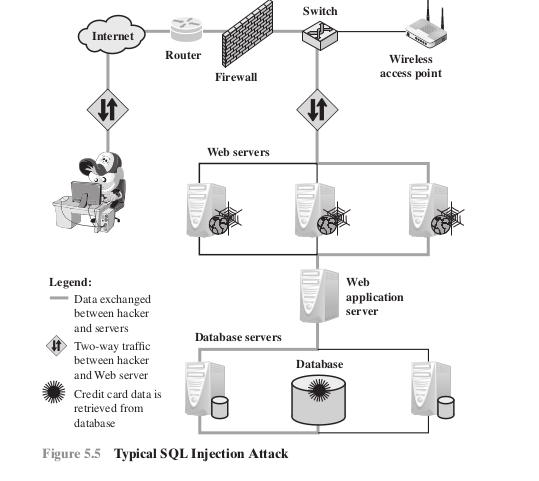
\includegraphics[width=14cm, keepaspectratio]{Bistarelli/img/cap_5/figura5.5.png}
\end{figure}


La Figura 5.5, tratta da, è un tipico esempio di attacco SQLi. I passi sono i seguenti:

\begin{enumerate}
    \item L'hacker trova una vulnerabilità in un'applicazione Web personalizzata e inietta un comando SQL in un database inviando il comando a un'applicazione Web. Il comando viene iniettato nel traffico che verrà accettato dal firewall.
    
    \item Il server Web riceve il codice dannoso e lo invia al server dell'applicazione Web.
    
    \item Il server delle applicazioni Web riceve il codice dannoso dal server Web e lo invia al server del database.
    
    \item  Il server del database esegue il codice dannoso sul database.
    
    Il database restituisce i dati della tabella delle carte di credito.
    
    \item  Il server dell'applicazione Web genera dinamicamente una pagina con i dati della carta di credito dal database.
    
    \item  Il server Web invia i dati della carta di credito all'hacker.
\end{enumerate}

\newpage
\subsection{Vie e tipi di attacco SQLi}

Possiamo caratterizzare gli attacchi SQLi in termini di vie di attacco e di tipo di attacco.

\singlespacing

Le principali vie di attacco sono le seguenti:

\begin{itemize}
    \item \textbf{Input dell'utente}
    
    In questo caso, gli aggressori iniettano comandi SQL fornendo input dell'utente opportunamente elaborati. Un'applicazione Web può leggere l'input dell'utente in diversi modi, a seconda dell'ambiente in cui viene distribuita. Nella maggior parte degli attacchi SQLi che hanno come obiettivo le applicazioni Web, l'input dell'utente proviene in genere da moduli inviati all'applicazione Web tramite richieste HTTP GET o POST. Le applicazioni Web sono generalmente in grado di accedere all'input dell'utente contenuto in queste richieste come accederebbero a qualsiasi altra variabile nell'ambiente. 
    
    \item \textbf{Variabili del server} 
    
    Le variabili del server sono un insieme di variabili che contengono intestazioni HTTP, intestazioni del protocollo di rete e variabili ambientali. Le applicazioni Web utilizzano queste variabili del server in vari modi, come la registrazione di statistiche di utilizzo e identificare le tendenze di navigazione. Se queste variabili vengono registrate in un database senza sanitizzazione, si potrebbe creare una vulnerabilità SQL injection.
    
    Poiché gli aggressori possono falsificare i valori inseriti nelle intestazioni HTTP e di rete, possono sfruttare questa vulnerabilità inserendo i dati direttamente nelle intestazioni. Quando la query per registrare la variabile del server viene inviata al database, l'attacco nell'intestazione falsificata viene attivato.
    
    \item \textbf{Iniezione di secondo ordine}
    
    L'iniezione di secondo ordine si verifica quando i meccanismi di prevenzione contro gli attacchi SQL injection sono incompleti. Nell'iniezione di secondo ordine, un utente malintenzionato potrebbe basarsi su dati già presenti nel sistema o nel database per scatenare un attacco di tipo SQL injection, per cui quando si verifica l'attacco, l'input che modifica la query per causare un attacco non proviene dall'utente, ma dal sistema stesso.
    
    \item \textbf{Cookie}
    
    Quando un client torna a un'applicazione Web, i cookie possono essere utilizzati per ripristinare le informazioni sullo stato del client. Poiché il client ha il controllo sui cookie, un aggressore potrebbe alterare i cookie in modo tale che, quando il server applicativo crea una query SQL basata sul contenuto del cookie, la struttura e la funzione della query vengano modificate.
    
    \item \textbf{Input fisico dell'utente}
    
    L'iniezione SQL è possibile fornendo input all'utente che costruisce un attacco al di fuori dell'ambito delle richieste Web. Questo input dell'utente può assumere sotto forma di codici a barre convenzionali, tag RFID o persino moduli cartacei che vengono scansionati con il riconoscimento ottico dei caratteri e trasmessi a un sistema di gestione di database.
\end{itemize}
I tipi di attacco possono essere raggruppati in tre categorie principali: inband, inferential e out-of-band. Un attacco inband utilizza lo stesso canale di comunicazione per iniettare codice SQL e recuperare i risultati. I dati recuperati vengono presentati direttamente nella pagina web dell'applicazione. I tipi di attacco inband includono i seguenti:
\begin{itemize}
    \item \textbf{Tautologia:} Questa forma di attacco inietta codice in una o più dichiarazioni condizionali in modo che siano sempre valutate come vere. 
    
    \item \textbf{Commento di fine riga:} Dopo aver iniettato del codice in un particolare campo, il codice legittimo che segue codice legittimo che segue viene annullato attraverso l'uso di commenti di fine riga. Un esempio esempio, aggiungere "- -" dopo gli input, in modo che le query rimanenti non vengano trattate come codice non vengono trattate come codice eseguibile, ma come commenti. L'esempio di tautologia precedente è è anch'esso di questa forma.
    
    \item \textbf{Query di tipo "piggybacked":} L'aggressore aggiunge ulteriori query oltre a quella prevista, aggiungendo l'attacco a una richiesta legittima. Questa tecnica si basa su configurazioni del server che consentono diverse query all'interno di un'unica stringa di codice. L'esempio riportato nella sezione precedente è di questo tipo.
\end{itemize}
Con un attacco inferenziale, non c'è un vero e proprio trasferimento di dati, ma l'aggressore è in grado di ricostruire le informazioni inviando particolari richieste e osservando il comportamento del sito web.
il comportamento risultante del server del sito web/database. 

\singlespacing

I tipi di attacco inferenziale includono i seguenti:
\begin{itemize}
    \centering
    \item \textbf{Query illegali/logicamente errate}
    
    Questo attacco consente a un aggressore di raccogliere informazioni importanti sul tipo e sulla struttura del database di backend di un'applicazione Web. L'attacco è considerato una fase preliminare di raccolta di informazioni per altri attacchi. La vulnerabilità sfruttata da questo attacco è che la pagina di errore predefinita restituita dai server applicativi è spesso eccessivamente descrittiva. Infatti, il semplice fatto che venga generato un messaggio di errore può spesso rivelare a un aggressore parametri vulnerabili/iniettabili.
    
    \item \textbf{Iniezione SQL cieca}
    
    L'iniezione SQL cieca consente agli aggressori di dedurre i dati presenti in un sistema di database anche quando il sistema è sufficientemente sicuro da non mostrare alcuna informazione errata all'aggressore. L'attaccante pone al server domande di tipo vero/falso. Se l'affermazione iniettata è vera, il sito continua a funzionare normalmente. Se l'affermazione risulta falsa, anche se non viene visualizzato alcun messaggio di errore descrittivo, la pagina differisce in modo significativo da quella normalmente funzionante.
\end{itemize}
In un attacco \textbf{out-of-band}, i dati vengono recuperati utilizzando un canale diverso (ad esempio, un'e-mail con i risultati della query). un'e-mail con i risultati della query e inviata al tester). Questo può essere Questo può essere utilizzato quando ci sono limitazioni nel recupero delle informazioni, ma la connettività in uscita dal dal server del database è debole.

\subsection{Contromisure per attacchi SQLi}

Poiché gli attacchi SQLi sono così diffusi, dannosi e variegati sia per modalità di attacco che per tipologia, una singola contromisura è insufficiente. È piuttosto necessario un insieme integrato di tecniche. Molti attacchi SQLi hanno successo perché gli sviluppatori hanno utilizzato pratiche di codifica poco sicure. Pertanto, la codifica difensiva è un modo efficace per ridurre drasticamente la minaccia di SQLi. 

\singlespacing

Esempi di codifica difensiva sono i seguenti:

\begin{itemize}
    \item \textbf{Pratiche di codifica difensiva manuale:} Una vulnerabilità comune sfruttata dagli attacchi SQLi è l'insufficiente convalida dell'input. La soluzione più semplice per eliminare queste per eliminare queste vulnerabilità è l'applicazione di pratiche di codifica difensiva adeguate. 
    
    Un esempio è il controllo del tipo di input, per verificare che gli input che devono essere numerici non contengano caratteri diversi dalle cifre. Questo tipo di tecnica può attacchi basati su errori di forzatura nel sistema di gestione del database.
    
    \singlespacing
    
    Un altro tipo di pratica di codifica è quella che esegue la corrispondenza dei modelli per cercare di distinguere un input normale da uno anormale.
    
    \item \textbf{Inserimento di query parametrizzate:} Questo approccio cerca di prevenire l'SQLi consentendo allo sviluppatore dell'applicazione di specificare in modo più accurato la struttura di una query di una query SQL e di passarle i parametri di valore separatamente, in modo tale che qualsiasi modo che l'utente non possa modificare la struttura della query.
    
    \item \textbf{SQL DOM:} SQL DOM è un insieme di classi che consente la valutazione automatica dei tipi di dati e l'escape.
    
    Questo approccio utilizza l'incapsulamento delle database per fornire un modo sicuro e affidabile di accedere ai database. Questo cambia il processo di creazione delle query da un processo sregolato che utilizza la concatenazione di stringhe a uno sistematico che utilizza un tipo di processo sistematico che utilizza un'API con controllo di tipo. All'interno dell'API, gli sviluppatori di codice, come il filtraggio dell'input e il controllo rigoroso del tipo di input dell'utente.
\end{itemize}

Sono stati sviluppati diversi metodi di rilevamento, tra cui i seguenti:
\begin{itemize}
    \item \textbf{Basato sulla firma:} Questa tecnica tenta di corrispondere a specifici schemi di attacco.
    
    Questo approccio deve essere costantemente aggiornato e potrebbe non funzionare contro gli attacchi auto-modificanti.
    
    \textbf{Basato sulle anomalie:} Questo approccio cerca di definire il comportamento normale e poi rilevare i modelli di comportamento al di fuori dell'intervallo normale. Un certo numero di approcci
\end{itemize}
\section{Controllo dell'accesso al database}
I DBMS commerciali e open-source forniscono in genere una capacità di controllo degli accessi per il database.
per il database. Il DBMS opera sulla base del presupposto che il sistema informatico che abbia autenticato ogni utente. Come ulteriore linea di difesa, il sistema informatico può utilizzare il sistema generale di controllo degli accessi per determinare se un utente può accedere al database nel suo complesso.

\singlespacing

Per gli utenti che sono stati autenticati e a cui è stato concesso l'accesso al database, un sistema di controllo dell'accesso al database fornisce una funzionalità specifica che controlla l'accesso a porzioni del database.

\singlespacing

I DBMS commerciali e open-source forniscono un controllo di accesso discrezionale o basato sui ruoli. In genere, un DBMS può supportare una serie di politiche amministrative, tra cui le seguenti:

\begin{itemize}
    \item \textbf{Amministrazione centralizzata:} Un piccolo numero di utenti privilegiati può concedere e revocare i diritti di accesso.

    \item \textbf{Amministrazione basata sulla proprietà:} Il proprietario (creatore) di una tabella può concedere e revocare i diritti di accesso alla tabella.
    
    \item \textbf{Amministrazione decentralizzata:} Oltre a concedere e revocare i diritti di accesso a una tabella, il proprietario della tabella può concedere e revocare i diritti di autorizzazione ad altri utenti, consentendo loro di concedere e revocare i diritti di accesso alla tabella.
\end{itemize}

Come ogni sistema di controllo degli accessi, un sistema di controllo degli accessi ai database distingue diversi diritti di accesso, tra cui creazione, inserimento, cancellazione, aggiornamento, lettura e scrittura. I diritti di accesso possono riguardare l'intero database, singole tabelle o righe o colonne selezionate all'interno di una tabella.
o colonne all'interno di una tabella. 

\subsection{Autorizzazioni a cascata}
L'opzione di concessione consente di far passare un diritto di accesso a cascata attraverso un certo numero di utenti. 
Consideriamo un diritto di accesso specifico e illustriamo il fenomeno della cascata nella Figura 5.6. La figura indica che Ann concede il diritto di accesso a Bob al tempo $t = 10$ e a Chris al tempo $t = 20$. Supponiamo che l'opzione di concessione sia sempre utilizzata. Pertanto, Bob è in grado di concedere il diritto di accesso a David al tempo $t = 30$. Chris concede in modo ridondante il diritto di accesso a David al tempo $t = 50$. Nel frattempo, David concede il diritto a Ellen, che a sua volta lo concede a Jim e successivamente David concede il diritto a Frank. Così come la concessione dei privilegi avviene a cascata da un utente all'altro utilizzando l'opzione grant, anche la revoca dei privilegi avviene a cascata. 

\singlespacing

Così, se Ann revoca il diritto di accesso a Bob e Chris, il diritto di accesso viene revocato anche a David, Ellen, Jim e Frank. Una complicazione sorge quando un utente riceve lo stesso diritto di accesso più volte, come accade nel caso di David. Supponiamo che Bob revochi il privilegio a David. David ha ancora il diritto di accesso perché gli è stato concesso da Chris a $t = 50$. Tuttavia, David ha concesso il diritto di accesso a un altro utente. Tuttavia, David ha concesso il diritto di accesso a Ellen dopo aver ricevuto il diritto, con opzione di concessione, da Bob ma prima di riceverlo da Chris. La maggior parte delle implementazioni prevede che in questa circostanza il diritto di accesso a Ellen e quindi a Jim venga revocato quando Bob revoca il diritto di accesso a David. Questo perché a $t = 40$, quando David ha concesso il diritto di accesso a Ellen, David aveva solo l'opzione di concessione da parte di Bob. La revoca del diritto da parte di Bob provoca la revoca di tutte le successive concessioni a cascata riconducibili esclusivamente a Bob tramite David. Poiché David ha concesso il diritto di accesso a Frank dopo che a David era stato concesso il diritto di accesso con opzione di concessione da Chris, il diritto di accesso a Frank rimane. Questi effetti sono mostrati nella parte inferiore della Figura 5.6.

\begin{figure}[H]
	\centering
    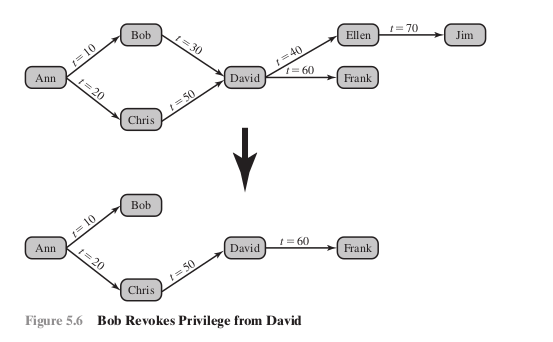
\includegraphics[width=14cm, keepaspectratio]{Bistarelli/img/cap_5/figura5.6.png}
\end{figure}


\begin{center}
    \textbf{Per generalizzare} la convenzione seguita dalla maggior parte delle implementazioni è la seguente. Quando l'utente A revoca un diritto d'accesso, viene revocato anche qualsiasi diritto d'accesso a cascata, a meno che a meno che quel diritto di accesso non esisterebbe anche se la concessione originale da parte di A non fosse mai avvenuta.
\end{center}

\subsection{Controllo dell'accesso basato sui ruoli}
Uno schema di controllo degli accessi basato sui ruoli (RBAC) si adatta naturalmente al controllo degli accessi ai database. A differenza di un file system associato a una o poche applicazioni, un sistema di database supporta spesso decine di applicazioni. In un ambiente di questo tipo, un singolo un singolo utente può utilizzare una serie di applicazioni per eseguire una varietà di compiti, ognuno dei quali richiede un proprio insieme di privilegi. Sarebbe una pratica amministrativa scorretta concedere semplicemente di concedere agli utenti tutti i diritti di accesso di cui hanno bisogno per tutte le attività che svolgono. RBAC fornisce un mezzo per alleggerire il carico amministrativo e migliorare la sicurezza.

\singlespacing

In un ambiente di controllo degli accessi discrezionale, si possono classificare gli utenti del database in tre grandi categorie in tre grandi categorie:

\begin{enumerate}
    \item \textbf{Proprietario dell'applicazione:} un utente finale che possiede oggetti di database (tabelle, colonne e righe) come parte di un'applicazione, e righe) come parte di un'applicazione. Cioè, gli oggetti del database sono generati dall'applicazione o sono preparati per essere utilizzati dall'applicazione.
    
    \item \textbf{Utente finale diverso dal proprietario dell'applicazione:} un utente finale che opera sugli oggetti del database attraverso una particolare applicazione, ma non base tramite una particolare applicazione, ma non possiede alcun oggetto del database.
    
    \item \textbf{Amministratore:} Utente che ha la responsabilità amministrativa di una parte o di tutto il database.
\end{enumerate}
È possibile fare alcune affermazioni generali su RBAC riguardo a questi tre tipi di utenti. Un'applicazione è associata a una serie di compiti, ognuno dei quali richiede diritti di accesso specifici a parti del database. ogni compito richiede diritti di accesso specifici a porzioni del database. Per ogni attività è possibile definire uno Per ogni attività è possibile definire uno o più ruoli che specificano i diritti di accesso necessari. 

\singlespacing

\paragraph{Il proprietario dell'applicazione dell'applicazione} può assegnare ruoli agli utenti finali. 

\singlespacing

\paragraph{Gli amministratori} sono responsabili dei ruoli più sensibili o generali, compresi quelli che hanno a che fare con la gestione dei componenti fisici e logici del database, come i file di dati, gli utenti e i meccanismi di sicurezza. Il sistema deve essere impostato in modo da dare a certi amministratori determinati privilegi. Gli amministratori, a loro volta, possono assegnare agli utenti ruoli di tipo amministrativo.

\singlespacing

Una struttura RBAC per database deve fornire le seguenti funzionalità:

\begin{itemize}
    \item Creare ed eliminare ruoli.
    
    \item Definire le autorizzazioni per un ruolo.
    
    \item Assegnare e annullare l'assegnazione degli utenti ai ruoli.
\end{itemize}
Un buon esempio dell'uso dei ruoli nella sicurezza dei database è la struttura RBAC di Microsoft SQL Server.

\singlespacing

SQL Server supporta tre tipi di ruoli: 

\begin{enumerate}

    \item Ruoli del server
    \item Ruoli del database 
    \item Ruoli definiti dall'utente.
    
\end{enumerate}

I primi due tipi di ruoli sono definiti ruoli fissi (vedere Tabella 5.2); sono preconfigurati per un sistema con diritti di accesso specifici. diritti di accesso specifici. L'amministratore o l'utente non possono aggiungere, eliminare o modificare i ruoli fissi; è possibile solo aggiungere e rimuovere utenti come è possibile solo aggiungere e rimuovere utenti come membri di un ruolo fisso. I ruoli fissi del server sono definiti a livello di server ed esistono indipendentemente da qualsiasi database di utenti. database degli utenti. Sono progettati per facilitare il compito amministrativo.

\begin{figure}[H]
	\centering
    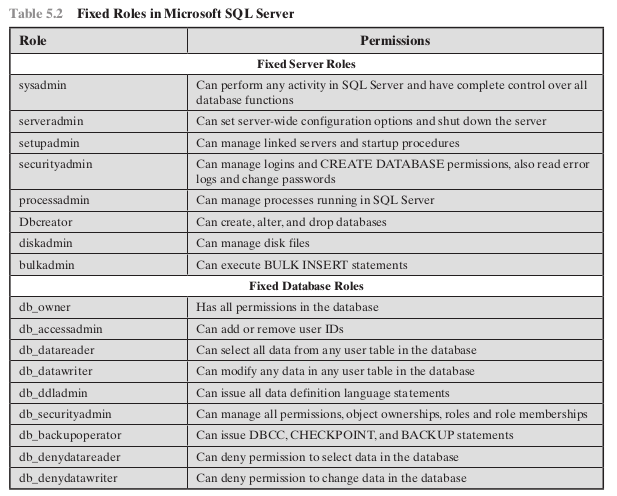
\includegraphics[width=14cm, keepaspectratio]{Bistarelli/img/cap_5/tabella5.2.png}
\end{figure}

Questi ruoli hanno autorizzazioni diverse e hanno lo scopo di fornire la possibilità di distribuire le responsabilità amministrative senza dover cedere il controllo completo. Gli amministratori di database possono usare questi ruoli fissi per assegnare diversi compiti amministrativi al personale e dare loro solo i diritti assolutamente necessari.
I ruoli fissi di database operano a livello di singolo database. Come nel caso dei ruoli di server fissi, alcuni ruoli di database fissi, come db\_accessadmin e db\_securityadmin, sono progettati per aiutare il DBA a delegare le responsabilità amministrative. Altri, come db\_datareader e db\_datawriter, sono stati progettati per fornire di autorizzazioni generali per un utente finale.

\singlespacing

Esistono due tipi di ruoli definiti dall'utente: Standard e Applicazione. 

\singlespacing

\paragraph{Per un ruolo standard} un utente autorizzato può assegnare altri utenti al ruolo.

\paragraph{Un ruolo applicativo} è associato a un'applicazione piuttosto che a un gruppo di utenti e richiede una password. Il ruolo viene attivato quando un'applicazione esegue il codice appropriato. Un utente che ha accesso all'applicazione può usare il ruolo di applicazione per accedere al database. Spesso le applicazioni di database applicano la propria sicurezza in base alla logica dell'applicazione. 

\singlespacing

Ad esempio, è possibile utilizzare un ruolo dell'applicazione con la propria password per consentire a un determinato utente di ottenere e modificare i dati solo in determinate ore. solo in determinati orari. In questo modo, è possibile realizzare una gestione della sicurezza più complessa all'interno della logica dell'applicazione.

\section{Interferenze}
L'inferenza, in relazione alla sicurezza dei database, è il processo di esecuzione di interrogazioni autorizzate e di deduzione di informazioni non autorizzate dalle risposte legittime ricevute.

\singlespacing

\begin{figure}[H]
	\centering
    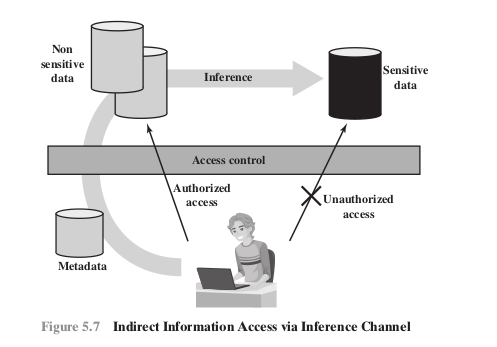
\includegraphics[width=14cm, keepaspectratio]{Bistarelli/img/cap_5/figura5.7.png}
\end{figure}

Il problema dell'inferenza si presenta quando la combinazione di un certo numero di dati è più sensibile dei singoli elementi, oppure quando una combinazione di dati può essere utilizzata per dedurre dati di maggiore sensibilità. La Figura 5.7 illustra il processo. L'attaccante può utilizzare sia i dati non sensibili sia i metadati. 

\singlespacing

I metadati si riferiscono alla conoscenza delle correlazioni o delle dipendenze tra i dati che possono essere utilizzate per dedurre informazioni non altrimenti disponibili a un particolare utente. Il percorso di trasferimento delle informazioni attraverso il quale si ottengono dati non autorizzati viene definito canale di inferenza.
In termini generali, si possono utilizzare due tecniche di inferenza per ricavare ulteriori informazioni aggiuntive: L'analisi delle dipendenze funzionali tra gli attributi all'interno di una tabella o tra le tabelle e l'unione di viste con gli stessi vincoli.

\singlespacing

Un esempio di quest'ultima tecnica, mostrato nella Figura 5.8, illustra il problema dell'inferenza. La Figura 5.8a mostra una tabella Inventario con quattro colonne. La Figura 5.8b mostra due viste, definite in SQL come segue:

\begin{figure}[H]
	\centering
    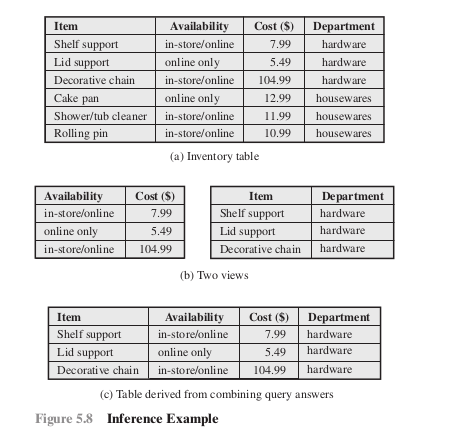
\includegraphics[width=14cm, keepaspectratio]{Bistarelli/img/cap_5/figura5.8.png}
\end{figure}

Gli utenti di queste viste non sono autorizzati ad accedere alla relazione tra Voce e Costo.
Un utente che ha accesso a una o a entrambe le viste non può dedurre la relazione attraverso le dipendenze funzionali. In altre parole, non esiste una relazione funzionale tra Articolo e Costo tale che la conoscenza dell'Articolo e forse di altre informazioni sia sufficiente per dedurre il Costo. Tuttavia, supponiamo che le due viste siano state create con il vincolo di accesso che Voce e Costo non possono essere consultati insieme. Un utente che conosce la struttura della tabella Inventario e che sa che le tabelle della vista mantengono lo stesso ordine delle righe della tabella Inventario è in grado di unire le due viste per costruire la tabella mostrata nella Figura 5.8c. In questo modo si viola la politica di controllo degli accessi, secondo cui la relazione tra gli attributi Item e Cost non deve essere divulgata.

\singlespacing

In termini generali, esistono due approcci per affrontare la minaccia della divulgazione per inferenza:

\begin{itemize}
    \item Rilevamento dell'inferenza durante la progettazione del database: Questo approccio rimuove un canale di inferenza modificando la struttura del database o cambiando il regime di controllo degli accessi per evitare l'inferenza.  Gli esempi includono la rimozione delle dipendenze di dati suddividendo una tabella in più tabelle o utilizzando ruoli di controllo dell'accesso a grana più fine in uno schema RBAC.

    \item Rilevamento delle inferenze al momento dell'interrogazione: Questo approccio cerca di eliminare una violazione del canale di inferenza
\end{itemize}
\newpage
\section{Crittografia del database}
Il database è in genere la risorsa informativa più preziosa per qualsiasi organizzazione ed è quindi protetto da più livelli di sicurezza, tra cui firewall, meccanismi di autenticazione, sistemi di controllo dell'accesso generale e sistemi di controllo dell'accesso al database. Inoltre, per i dati particolarmente sensibili, la crittografia del database è giustificata e spesso implementata. La crittografia diventa l'ultima linea di difesa nella sicurezza dei database.

\singlespacing

La crittografia dei database presenta due svantaggi:

\begin{enumerate}
    \item \textbf{Gestione delle chiavi}
    
    Gli utenti autorizzati devono avere accesso alla chiave di decifrazione per i dati a cui hanno accesso. per i dati ai quali hanno accesso. Poiché un database è tipicamente accessibile a un'ampia gamma di utenti e di applicazioni, è necessario fornire chiavi sicure a parti selezionate del database. 
    
    \item \textbf{Inflessibilità}
    
    Quando una parte o la totalità del database è crittografata, diventa più difficile eseguire la ricerca dei record. La crittografia può essere applicata all'intero database, a livello di record (crittografia di record record selezionati), a livello di attributi (crittografia di colonne selezionate) o a livello di singoli campi.
    
\end{enumerate}
Sono stati adottati diversi approcci alla crittografia dei database. In questa sezione, esaminiamo un approccio rappresentativo per un database multiutente. Un DBMS è un complesso insieme di hardware e software. Richiede una grande
capacità di memorizzazione e richiede personale qualificato per la manutenzione, la protezione dai disastri, l'aggiornamento e la sicurezza.

Per molte organizzazioni di piccole e medie dimensioni, una soluzione interessante è quella di esternalizzare il DBMS e il database a un fornitore di servizi. Il fornitore di servizi gestisce il database fuori sede e può garantire un'elevata disponibilità, la prevenzione dei disastri e un accesso e un aggiornamento efficienti. Il problema principale di questa soluzione è la riservatezza dei dati.

\singlespacing

Una soluzione semplice al problema della sicurezza in questo contesto è quella di crittografare l'intero database e non fornire la crittografia dell'intero database e non fornire le chiavi di crittografia/decrittografia al fornitore di servizi. Questa soluzione è di per sé poco flessibile. L'utente non ha la possibilità di accedere a singoli dati in base a ricerche o indicizzazioni su parametri chiave, ma deve scaricare intere tabelle dal database, decifrarle e lavorare con i risultati. 

\singlespacing

Per garantire una maggiore flessibilità, deve essere possibile lavorare con il database nella sua forma criptata. Un esempio di questo tipo di approccio, illustrato nella Figura 5.9. Un approccio simile è descritto in [HACI02]. Le entità coinvolte sono quattro coinvolte:

\begin{enumerate}
    \item \textbf{Proprietario dei dati:} un'organizzazione che produce dati da rendere disponibili per il rilascio controllato, sia all'interno dell'organizzazione che all'esterno.
    
    \item  \textbf{Utente:} entità umana che presenta richieste (query) al sistema. L'utente può essere un dipendente dell'organizzazione a cui viene concesso l'accesso al database tramite il server, oppure un utente esterno.
    
    \item \textbf{Client:} Front-end che trasforma le interrogazioni dell'utente in interrogazioni sui dati crittografati memorizzati sul server.
    
    \item \textbf{Server:} Un'organizzazione che riceve i dati crittografati da un proprietario di dati e li rende disponibili per la distribuzione ai clienti.
    
    Il server può essere di fatto di proprietà del proprietario dei dati ma, più tipicamente, è una struttura posseduta e gestita da un fornitore esterno. 
\end{enumerate}

Inserire figura 5.9 

Esaminiamo innanzitutto la soluzione più semplice possibile basata su questo scenario. Supponiamo che ogni singolo elemento del database sia crittografato separatamente, utilizzando la stessa chiave di crittografia.
Il database crittografato è memorizzato sul server, ma il server non possiede la chiave, quindi i dati sono al sicuro sul server. Anche se qualcuno fosse in grado riuscire a penetrare nel sistema del server, avrebbe accesso solo ai dati crittografati. dati crittografati. Il sistema client dispone di una copia della chiave di crittografia. Un utente del client può recuperare un record dal database con la seguente sequenza:

\begin{enumerate}
    \item L'utente esegue una query SQL per i campi di uno o più record con un valore specifico della chiave primaria.
    
    \item Il processore di query del client cripta la chiave primaria, modifica la query SQL di conseguenza e la trasmette al server.
    
    \item Il server elabora la query utilizzando il valore criptato della chiave primaria e restituisce il record o i record appropriati.
    
    \item L'elaboratore della query decifra i dati e restituisce i risultati.
\end{enumerate}
\newpage
\section{Sicurezza dei data center}
Un data center è una struttura aziendale che ospita un gran numero di server, dispositivi di archiviazione, switch e apparecchiature di rete. Il numero di server e dispositivi di archiviazione può raggiungere le decine di migliaia in una singola struttura. 

\singlespacing

Esempi di utilizzo di questi grandi data center sono i fornitori di servizi cloud, i motori di ricerca, le grandi strutture di ricerca scientifica e le strutture IT per le grandi aziende. Un data center generalmente include alimentatori ridondanti o di backup, connessioni di rete ridondanti, controlli ambientali (ad esempio, aria condizionata e soppressione degli incendi) e vari dispositivi di sicurezza. dispositivi di sicurezza. I data center di grandi dimensioni sono operazioni su scala industriale che utilizzano l'energia elettrica come una piccola città. Un data center può occupare una stanza di un edificio, uno o più piani, o un intero edificio.

\subsection{Elementi dei data center}

\begin{figure}[H]
	\centering
    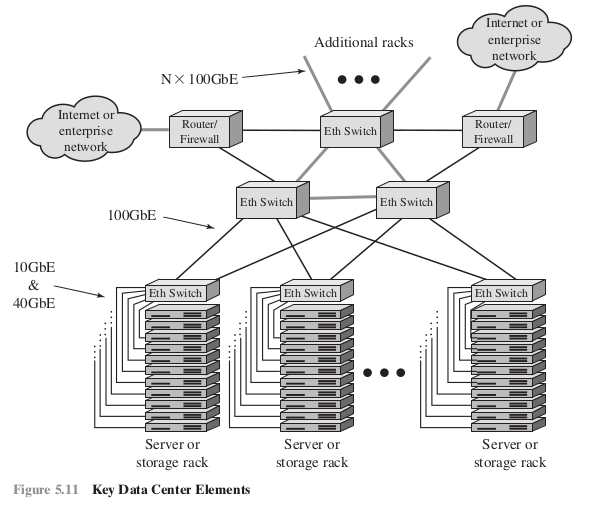
\includegraphics[width=14cm, keepaspectratio]{Bistarelli/img/cap_5/figura5.11.png}
\end{figure}

La Figura 5.11 illustra gli elementi chiave della configurazione di un grande data center. La maggior parte delle apparecchiature di un grande data center è costituita da pile di server e moduli di archiviazione montati in rack aperti o armadietti chiusi, che di solito sono disposti in file singole con corridoi tra di loro. Ciò consente l'accesso alla parte anteriore e posteriore di ciascun rack o armadio. In genere, i singoli moduli sono dotati di porte Ethernet da 10 o 40 Gbps per gestire il traffico massiccio da e verso i server. Inoltre, ogni rack è dotato di uno o due switch Ethernet da 10, 40 o 100 Gbps per interconnettere tutti i server e fornire connettività al resto della struttura. Gli switch sono spesso montati nel rack e vengono definiti switch top-of-rack (ToR). Il termine ToR è diventato sinonimo di switch di accesso al server, anche se non si trova "top of rack". I data center di grandi dimensioni, come i provider di cloud, richiedono switch che operano a 100 Gbps per supportare l'interconnessione dei rack di server e fornire una capacità adeguata per la connessione fuori sede tramite controller di interfaccia di rete (NIC) su router o firewall. o firewall. 

\singlespacing

Gli elementi chiave non mostrati nella Figura 5.11 sono il cablaggio e le connessioni incrociate, che possiamo elencare come segue.

\begin{itemize}
    \item \textbf{Cross connect:} Una struttura che consente la terminazione dei cavi, nonché la loro interconnessione con altri cavi o apparecchiature.
    
    \item \textbf{Cablaggio orizzontale:} Qualsiasi cablaggio utilizzato per collegare l'armadio di cablaggio di un piano alle piastre a muro nelle aree di lavoro per fornire le linee della rete locale (LAN) per collegare server e altre apparecchiature digitali alla rete. Il termine orizzontale è usato perché questo tipo di cablaggio è in genere eseguito lungo il soffitto o il pavimento.
    
    \item \textbf{Cablaggio backbone:} Eseguito tra le stanze o gli armadi del data center e il punto di collegamento principale di un edificio.

\end{itemize}
\subsection{Considerazioni sulla sicurezza dei data center}
Tutte le minacce alla sicurezza e le contromisure discusse in questo testo sono rilevanti nel contesto dei grandi centri dati. Nel contesto dei grandi centri di elaborazione dati, ed è infatti in questo contesto che i rischi
sono più acuti.

\singlespacing

Si consideri che il data center ospita enormi quantità di dati che sono:

\begin{itemize}
    \item Situati in uno spazio fisico limitato.
    
    \item Interconnessi con cablaggi a connessione diretta.
    
    \item Accessibili attraverso connessioni di rete esterne, per cui una volta superato il confine, una  minaccia per l'intero complesso.
    
    \item Tipicamente rappresentano la più grande risorsa dell'azienda.
\end{itemize}
Pertanto, la sicurezza dei data center è una priorità assoluta per qualsiasi azienda con un data center di grandi dimensioni.

\singlespacing

Alcune delle minacce più importanti da considerare sono le seguenti:

\begin{itemize}
    \item Negazione del servizio
    
    \item Minacce persistenti avanzate da attacchi mirati
    
    \item Violazioni della privacy
    
    \item Sfruttamenti di applicazioni come l'iniezione di SQL
    
    \item Malware
    
    \item Minacce alla sicurezza fisica
\end{itemize}

\begin{figure}[H]
	\centering
    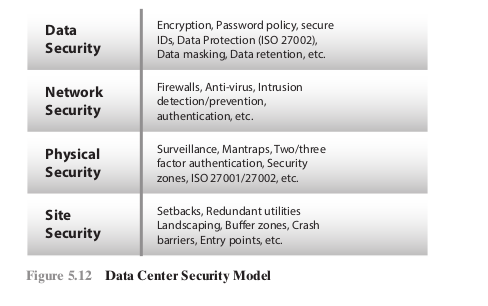
\includegraphics[width=14cm, keepaspectratio]{Bistarelli/img/cap_5/figura5.12.png}
\end{figure}

La Figura 5.12 mette in evidenza gli aspetti importanti della sicurezza dei data center, rappresentati come un modello a quattro livelli. La sicurezza del sito si riferisce principalmente alla sicurezza fisica dell'intero sito, compreso l'edificio che ospita il data center. La sicurezza fisica del data center stesso comprende barriere all'ingresso, come ad esempio una all'ingresso, come ad esempio un mantra (uno spazio di controllo dell'accesso a due porte per una sola persona) e tecniche di autenticazione per ottenere l'accesso fisico. La sicurezza della rete è estremamente importante in una struttura in cui un insieme così ampio di risorse è concentrato in un unico luogo e accessibile da connessioni di rete esterne. 
\subsection{TIA-492}
Lo standard TIA (Telecommunications Industry Association) TIA-492 (Telecommunications Infrastructure Standard for Data Centers) specifica i requisiti minimi per le infrastrutture di telecomunicazione dei data center. 

\singlespacing

Questa architettura anticipa la crescita e contribuisce a creare un ambiente in cui le applicazioni e i server possono
e server possono essere aggiunti e aggiornati con tempi di inattività minimi. Questo approccio standardizzato
Questo approccio standardizzato supporta l'alta disponibilità e un ambiente uniforme per l'implementazione di misure di sicurezza. 

\begin{figure}[H]
	\centering
    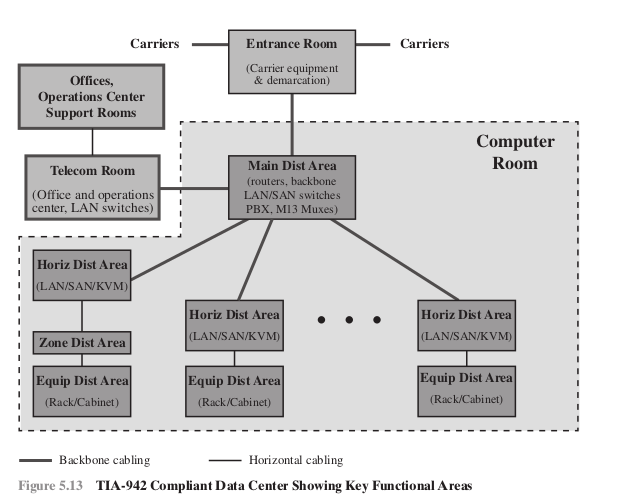
\includegraphics[width=14cm, keepaspectratio]{Bistarelli/img/cap_5/figura5.13.png}
\end{figure}

\singlespacing

La norma TIA-942 specifica che un data center dovrebbe includere le seguenti aree funzionali (vedi Figura 5.13).

\begin{itemize}
    \item \textbf{Sala computer:} Porzione del data center che ospita le apparecchiature di elaborazione dati.
    
    \item \textbf{Sala d'ingresso:} Una o più sale d'ingresso ospitano le apparecchiature esterne del di accesso alla rete esterna e forniscono l'interfaccia tra le apparecchiature della sala computer e i sistemi di cablaggio dell'azienda. e i sistemi di cablaggio aziendali. La separazione fisica della sala d'ingresso dalla sala computer sala d'ingresso dalla sala computer garantisce una maggiore sicurezza.
    
    \item \textbf{Area di distribuzione principale:} Un'area centrale che ospita il collegamento trasversale principale e i router e gli switch principali per le infrastrutture LAN e SAN (storage area network).
    
    \item \textbf{Area di distribuzione orizzontale (HDA):} Serve come punto di distribuzione per il cablaggio orizzontale e ospita le connessioni incrociate e le apparecchiature attive per la distribuzione dei cavi all'area di distribuzione delle apparecchiature.
    
    \item \textbf{Area di distribuzione delle apparecchiature (EDA):} L'ubicazione degli armadietti delle apparecchiature e dei rack, con cavi orizzontali che terminano con pannelli patch.
    
    \item \textbf{Area di distribuzione di zona (ZDA):} Un punto di interconnessione opzionale nel cablaggio orizzontale tra l'HDA e l'EDA. La ZDA può fungere da punto di consolidamento come punto di consolidamento per la flessibilità di riconfigurazione o per l'alloggiamento di apparecchiature indipendenti come come i mainframe.
\end{itemize}
